\documentclass[tikz,border=5pt]{standalone}
\usepackage{tikz}
\usetikzlibrary{decorations.pathreplacing} % Required for the brace

\usetikzlibrary{shapes.symbols, shapes.geometric, arrows.meta, positioning}

% 2. Define the styles used in your diagram
\tikzset{
    block/.style = {rectangle, draw, fill=blue!10, text width=10em, text centered, rounded corners, minimum height=2em},
    cloud/.style = {draw, ellipse, fill=red!10, node distance=3cm, minimum height=2em},
    arrow/.style = {thick, ->, >=stealth}
    ellipse/.style={
        ellipse,           % The actual shape
        draw=black,        % Border color
        fill=blue!10,      % Background color
        thick,             % Border thickness
        minimum width=3cm, % Minimum horizontal size
        minimum height=2cm % Minimum vertical size
    }
}

\begin{document}

% Adjust scale=... to fit your slide.
% scale=0.6 usually works well within a standard Beamer frame column.
    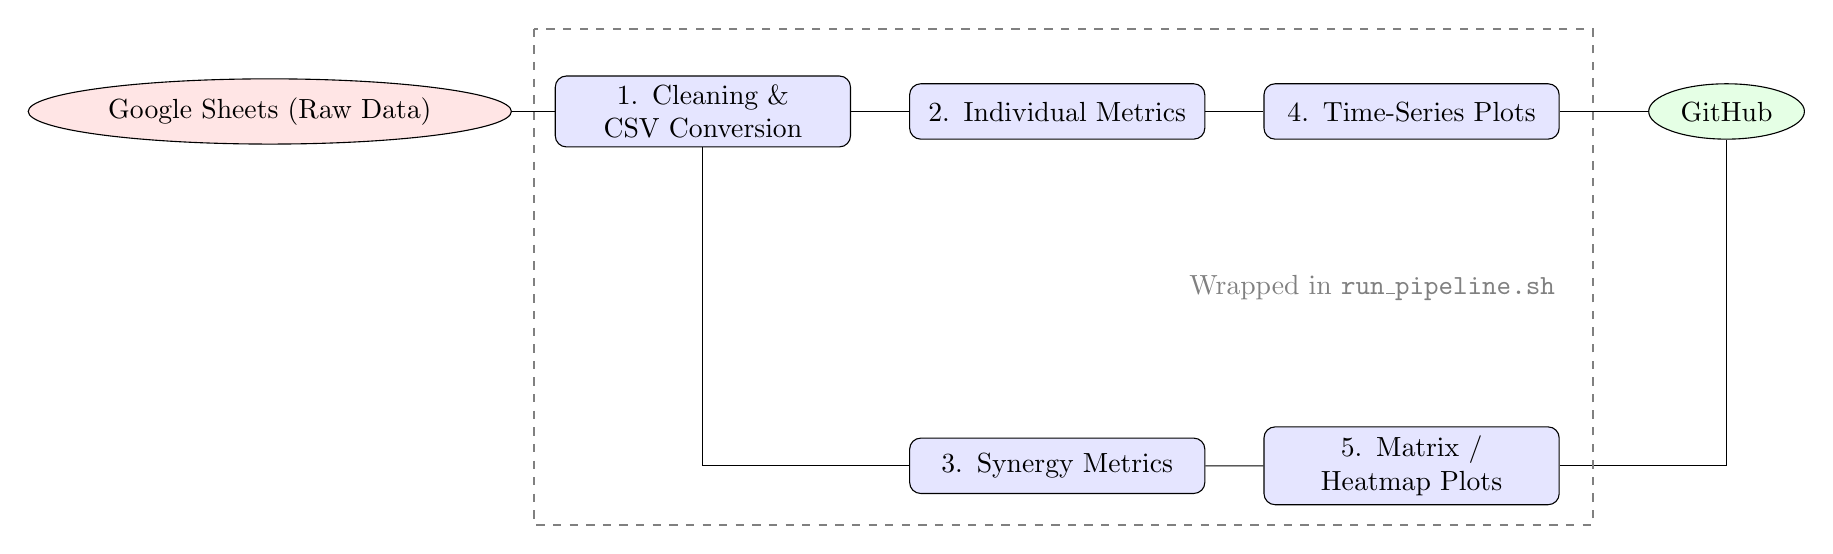
\begin{tikzpicture}[node distance = 2cm, auto, scale=0.7, >=stealth]
        % Nodes
        \node [cloud] (google) {Google Sheets (Raw Data)};
        \node [block, right of=google, node distance=5.5cm] (clean) {1. Cleaning \& CSV Conversion};
        \node [block, right of=clean, node distance=4.5cm] (indiv) {2. Individual Metrics};
        \node [block, below of=indiv, node distance=4.5cm] (synergy) {3. Synergy Metrics};
        \node [block, right of=indiv, node distance=4.5cm] (plot1) {4. Time-Series Plots};
        \node [block, right of=synergy, node distance=4.5cm] (plot2) {5. Matrix / Heatmap Plots};
        \node [cloud, right of=plot1, node distance=4cm, fill=green!10] (github) {GitHub};

        % Edges
        \draw [arrow] (google) -- (clean);
        \draw [arrow] (clean) -- (indiv);
        \draw [arrow] (clean) |- (synergy);
        \draw [arrow] (indiv) -- (plot1);
        \draw [arrow] (synergy) -- (plot2);
        \draw [arrow] (plot1) -- (github);
        \draw [arrow] (plot2) -| (github);
        
        % Automation Wrapper
        \draw[dashed, thick, gray] (4.8,1.5) rectangle (24., -7.5);
        \node[text=gray] at (20, -3.2) {Wrapped in \texttt{run\_pipeline.sh}};

    \end{tikzpicture}
\end{document}